\documentclass{beamer}

\mode<presentation>
{
  \usetheme{Pittsburgh}
  \useoutertheme{split}
  \setbeamercovered{transparent} 
  \setbeamertemplate{navigation symbols}{}
  \setbeamertemplate{title}{}
  % \setbeamertemplate{footline}[page number]{}
  % \setbeamertemplate{footline}[frame number]
}

\usepackage{amsmath}
\usepackage[english]{babel}
\usepackage[utf8]{inputenc}
\usepackage{times}
\usepackage[T1]{fontenc}
\usepackage{graphicx}
\usepackage{hyperref}
\usepackage{subfigure}
\usepackage{setspace}
\usepackage{multirow}
\usepackage{booktabs}
\usepackage{tabulary}
\usepackage{tabu}

\title[Introduction: Social Data Analytics]
{Introduction: Social Data Analytics}

\author{INF1005/6, Prof. Alex Hanna}
\institute[] {
}

\date[] {
January 12, 2017
}

\begin{document}

\begin{frame}
  \titlepage
\end{frame}

\begin{frame}{Class Description}
    \begin{itemize}
        \item ``Big (Social) Data''
        \item Data Ethics
        \item Computer programming
    \end{itemize}
\end{frame}

\begin{frame}{Class Goals}
  \begin{columns}
    \begin{column}{0.5\textwidth}
      \begin{itemize}[<+->]
        \item Identify
        \item Collect
        \item Transform
        \item Analyze
        \item Visualise
      \end{itemize}
    \end{column}
    \begin{column}{0.5\textwidth}
      \only<1>{\includegraphics[width=\textwidth]{img/identify-data.png}}
      \only<2>{\includegraphics[width=\textwidth]{img/collect-data.png}}
      \only<3>{\includegraphics[width=\textwidth]{img/transform-data.png}}
      \only<4>{\includegraphics[width=\textwidth]{img/analyze-data.png}}
      \only<5>{\includegraphics[width=\textwidth]{img/visualise-data.png}}
    \end{column}
  \end{columns}
\end{frame}

\begin{frame}{Class Requirements}
  \begin{center}
      \begin{itemize}[<+->]
        \item Attendance (20\%)
        \item Assignment 1 (40\%)
        \item Assignment 2 (40\%)
      \end{itemize}
  \end{center}
\end{frame}

\begin{frame}{Procedures and Rules}
    \begin{itemize}[<+->]
        \item E-Culture 
        \item Academic integrity
        \item Equity and diversity
    \end{itemize}
\end{frame}


\begin{frame}{About Me}
  \begin{columns}
    \begin{column}{0.5\textwidth}
        \begin{itemize}[<+->]
          \item Professor Alex Hanna (Prof. Hanna, or Dr. Hanna)
          \item PhD and MS in Sociology
          \item BS in Computer Science
          \item Transgender and queer
          \item Pronouns: she/her/hers
          \only<6>{\item Roller derby player/announcer/coach}
        \end{itemize}
    \end{column}
    \begin{column}{0.5\textwidth}
        \only<6>{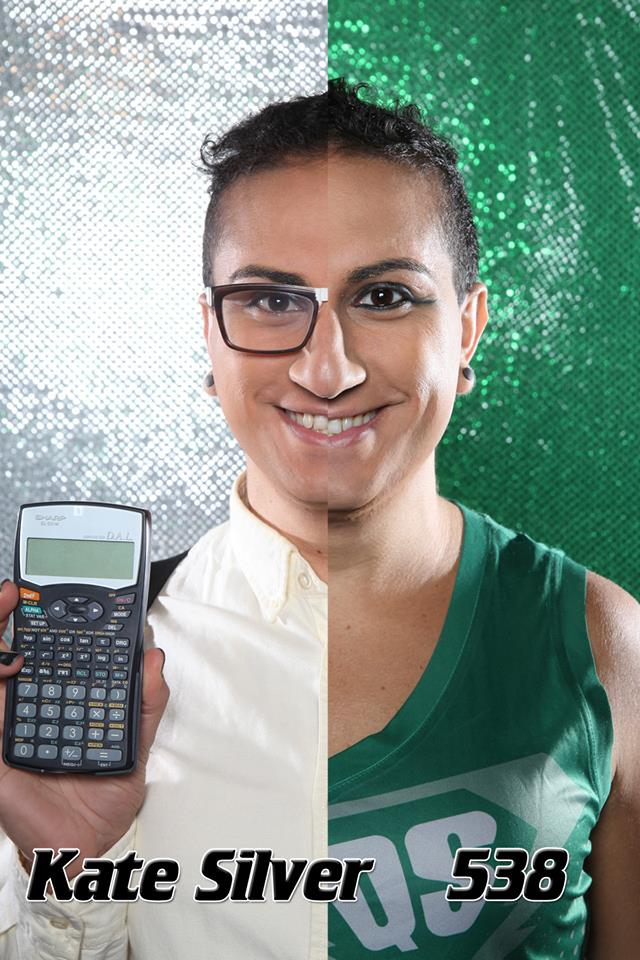
\includegraphics[width=0.9\textwidth]{img/ks-calc.jpg}}
    \end{column}
  \end{columns}
\end{frame}

\begin{frame}{About You!}
  \centering
  \url{http://bit.ly/inf1005-survey}
\end{frame}

\begin{frame}[plain]
  \begin{center}
    \bf \LARGE What are Social Data Analytics?
  \end{center}
\end{frame}

\begin{frame}[plain]
  \begin{center}
      
\includegraphics[width=0.5\textwidth]{img/instagram-logo.png} \\
      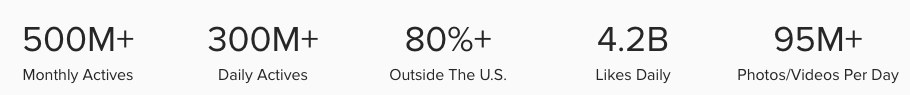
\includegraphics[width=\textwidth]{img/instagram-stats.png} \\
  \end{center}
\end{frame}

\begin{frame}[plain]
  \begin{center}
      
\includegraphics[width=0.5\textwidth]{img/twitter-logo.png} \\
      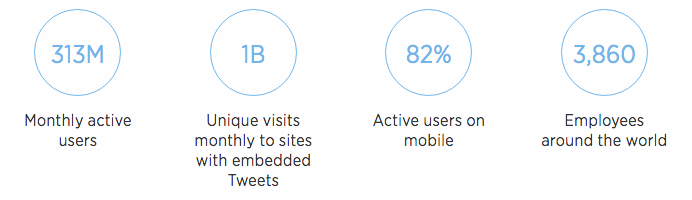
\includegraphics[width=\textwidth]{img/twitter-stats.png} \\
  \end{center}
\end{frame}

\begin{frame}[plain]
  \begin{center}
      
\includegraphics[width=0.5\textwidth]{img/shopify-logo.png} \\

      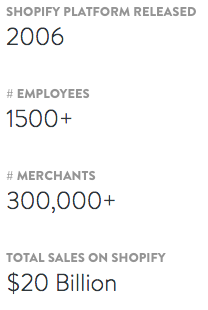
\includegraphics[width=0.4\textwidth]{img/shopify-stats.png}
  \end{center}
\end{frame}

\begin{frame}[plain]
  \begin{center}
      
\includegraphics[width=0.5\textwidth]{img/stats-can.png} \\
      Five-year Census of every Canadian (>35 million) \\
      350+ active surveys on Canadian life
  \end{center}
\end{frame}

\begin{frame}{Big Data is ``Trace'' Data}
  \begin{center}
    \includegraphics[width=0.65\textwidth]{img/traces.png} 
  \end{center}
\end{frame}

\begin{frame}{Big Data Fields}
    \begin{center}
        ``Data Science'' \\
        ``Business intellgence and analytics'' \\
        ``Computational social science''
    \end{center}
\end{frame}

\begin{frame}[plain]
  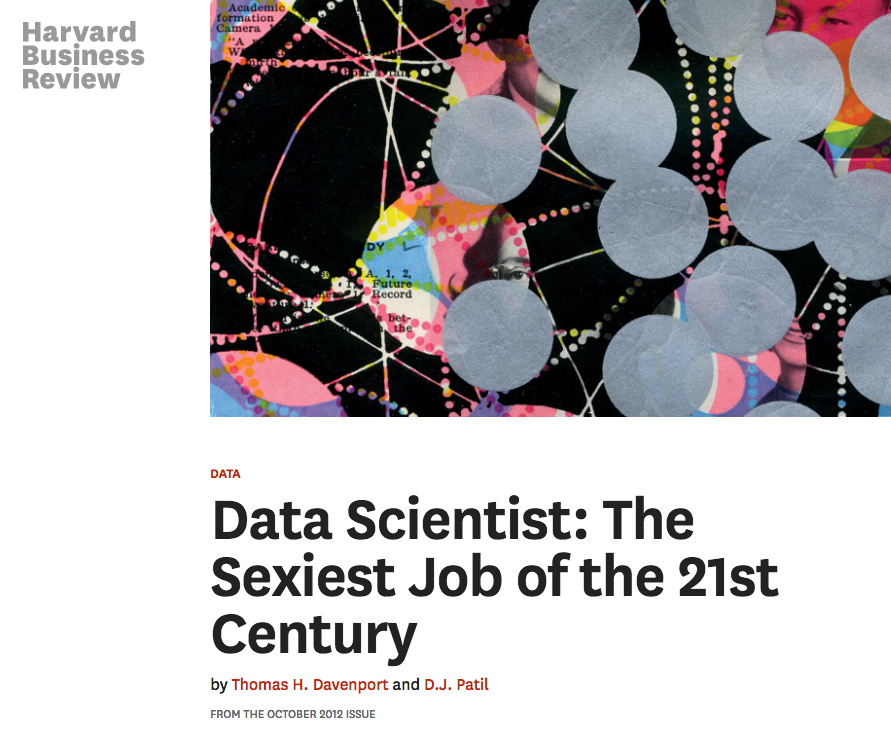
\includegraphics[width=\paperwidth]{img/data-science-hbr-sexy.png}
\end{frame}

\begin{frame}{Computational Social Science (Shah et al. 2015)}
  \begin{itemize}[<+->]
    \item the use of large, complex datasets, often... measured in terabytes or petabytes
    \item the frequent involvement of `naturally occurring' social and digital media sources and other electronic databases
    \item the use of computational or algorithmic solutions to generate patterns and inferences from these data
    \item the applicability to social theory in a variety of domains from the study of mass opinion to public health, from examinations of political events to social movements
  \end{itemize}
\end{frame}

\begin{frame}{Computational Social Science}
  \begin{columns}
    \begin{column}{0.5\textwidth}    
      \begin{itemize}[<+->]
        \item Network analysis
        \item Automated content (e.g. text and image) analysis
        \item Massive Online Experiments
       \end{itemize}
    \end{column}
    \begin{column}{0.5\textwidth}
      \only<1>{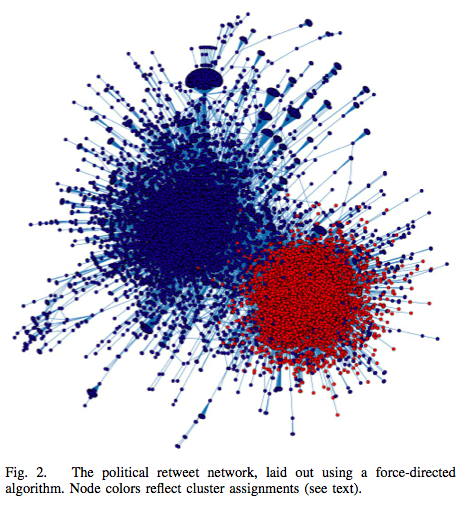
\includegraphics[width=\textwidth]{img/conover_etal-f2.png}}
      \only<2>{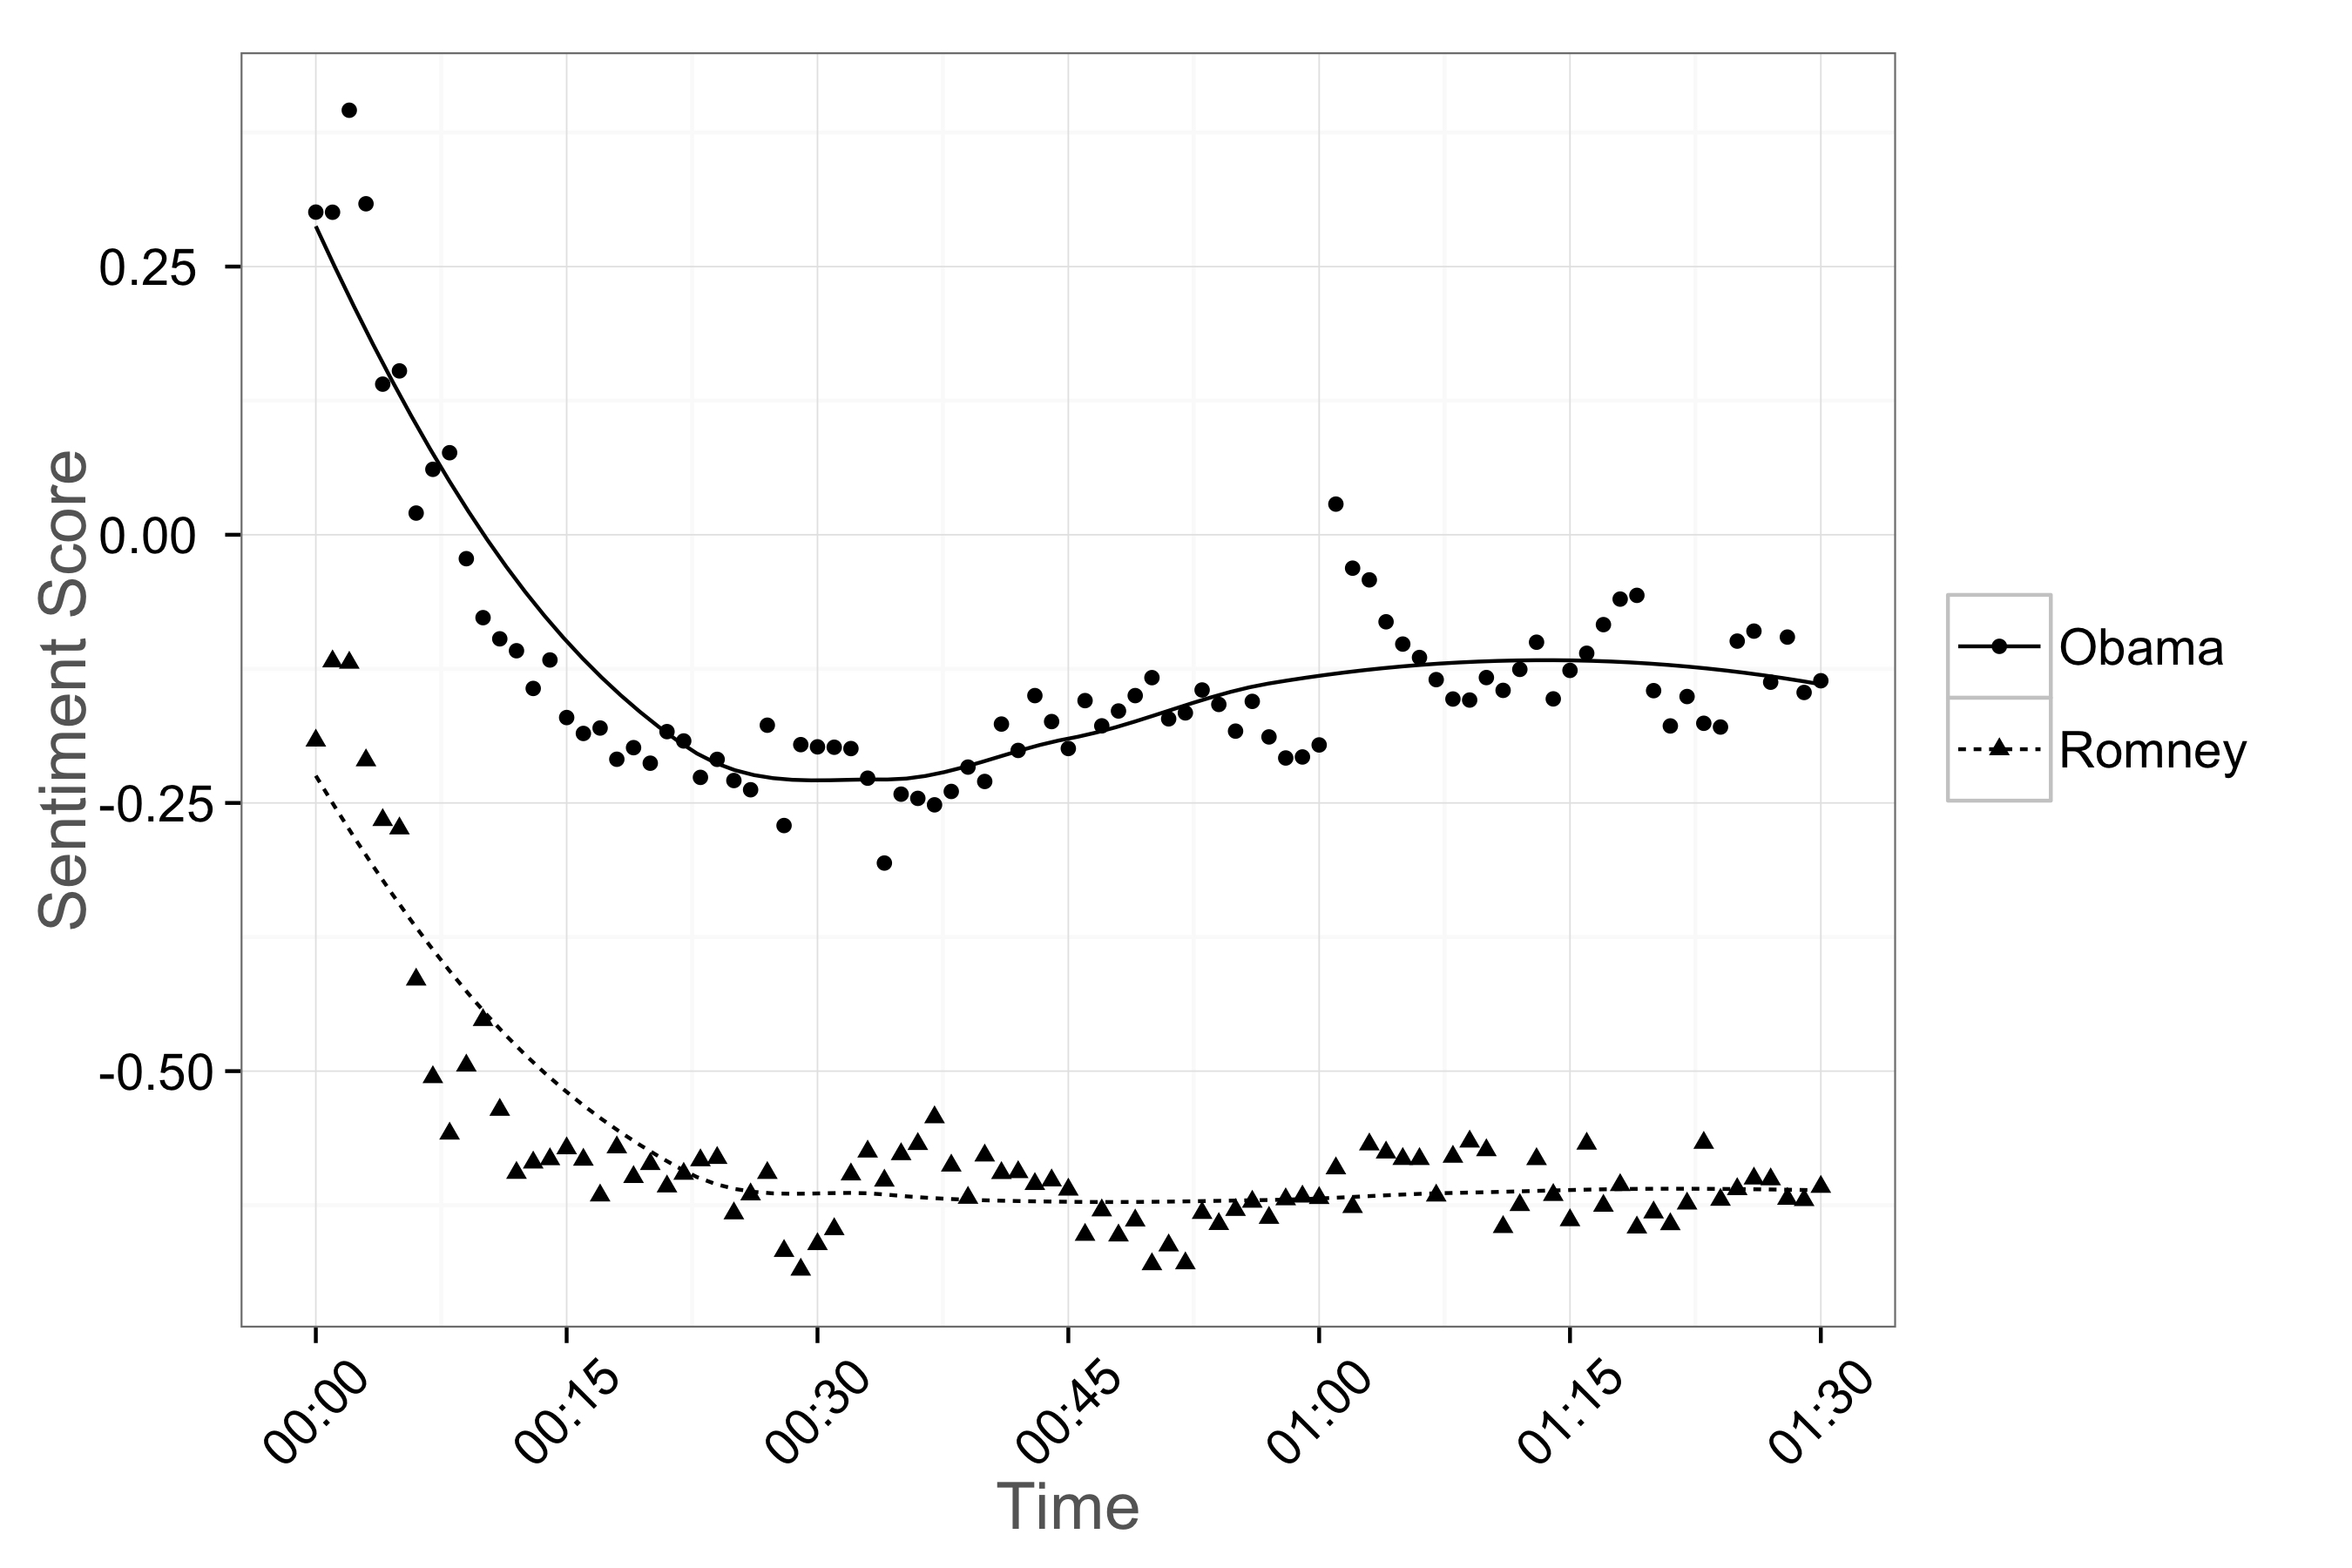
\includegraphics[width=\textwidth]{img/gh-usprez.jpg}}
      \only<3>{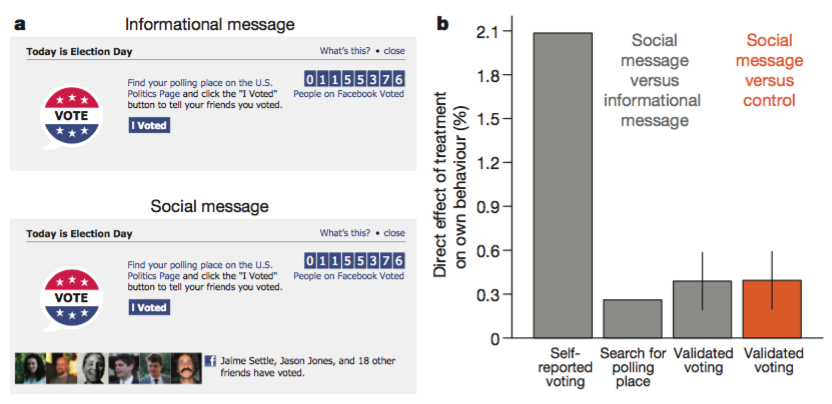
\includegraphics[width=\textwidth]{img/bond_etal-f1.png}}
    \end{column}
  \end{columns}
\end{frame}

\begin{frame}{Big Data Gone Wrong: Google Flu Trends}
  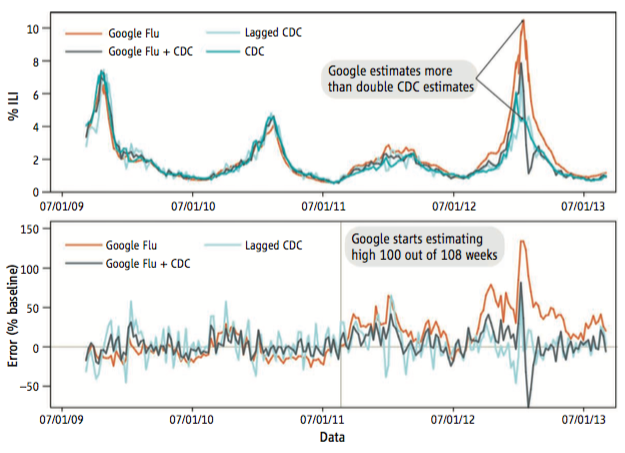
\includegraphics[width=0.9\textwidth]{img/lazer_etal_2014-f1.png}
\end{frame}

\begin{frame}{Big Data Gone Wrong: Facebook and Emotions}
  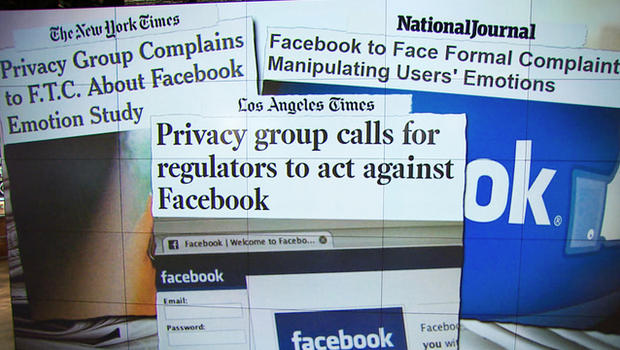
\includegraphics[width=\textwidth]{img/fb-emotion-study.jpg}
\end{frame}

\begin{frame}{Coding as Thinking}
    \begin{itemize}
        \item Programming languages get old, thinking does not
        \item When you program, you open doors
        \begin{itemize}
          \item DIY
          \item Troubleshooting
          \item Career
        \end{itemize}
    \end{itemize}
\end{frame}

\begin{frame}[plain]
    
\includegraphics[width=\textwidth]{img/python-logo.jpg}
\end{frame}

% \begin{frame}{Transparency and Replicability}
%     Git, open-source, data sharing
% \end{frame}

% \begin{frame}[plain]
%     \begin{center}
%       \bf \LARGE Programming (thinking) exercise: How to program a computer
%     \end{center}
% \end{frame}

% \begin{frame}{Topics to Cover in Class}
    
% \end{frame}

\end{document}
